\section{Übungsaufgaben: Asymmetrische Kryptologie}
\subsection{Rucksack}
\subsection{RSA auf Nachricht in Blöcken}


\begin{align}
  P &= \text{'FHT4EVER'}  &
  n &= 13 \cdot 17 = 221 & e &= 3
\end{align}

\textbf{Beachten: $ggT(e, \phi(221) ) \ne 1$}. Entschlüsselung damit ummöligch.

\begin{align}
	E(x) &=  x^3 \mod 221 \\
	E(P) &=  E('F') \circ E('H')\circ E('T')\circ E('4')\circ E('E')\circ E('V')\circ E('E')\circ E('R')\\
		 &=  \operatorname{apply}(x^3 \mod 221 ,[70, 72, 84, 52, 69, 86, 69, 82])    \\
		 &=  [8, 200, 203, 52, 103, 18, 103, 194]
\end{align}


\subsection{Chinesischer Restsatz}
\subsubsection{Es sei $m = 11, n = 12, a = 3$ und $b = 4$. Geben Sie ein $x$ an, für das gilt: $x \mod m = a$ und $ x \mod n = b$}

\begin{equation}
	x = a n N + b m M  = 3 \cdot 12 \cdot N + 4 \cdot 11 M
\end{equation}

$$ggT(12, 11) = 1 \text{ mit } a^{-1} = -1 = N$$
$$ggT(11, 12) = 1 \text{ mit } a^{-1} =  1 = M$$

\begin{align}
	X &= 3 \cdot 12 \cdot 1 + 4 \cdot 11 \cdot -1 \\
	  &=  36 - 44 = -8
\end{align}
\textbf{Probe:}
\begin{align}
	-8 \mod  m &= a  & -8 \mod  n &= b \\
	-8 \mod 11 &= 3  & -8 \mod 12 &= 4 \\
\end{align}

\subsubsection{Es sei $m = 11, n = 12, l = 12, a = 3, b = 4 \text{ und } c=5$. Geben Sie ein $x$ an, für das
gilt: $x \mod m = a$ und $x \mod n = b$ und $x \mod l = c$.}

\begin{align}
 X = a \cdot n \cdot l (nl)^{-1}
   + b \cdot m \cdot l (ml)^{-1}
   + c \cdot n \cdot m (nm)^{-1}
\end{align}

\textbf{Vorrausetzung für Chin. Restsatz nicht erfüllt.}
$ggT(n,l)=12$ damit nicht relativ prim.

\subsubsection{Verallgemeinern Sie den Chinesischer Restsatz:
Gesucht ist $x$ mit $(x \mod m_i)=x_i$ und die passende Berechnungsvorschrift. Wie groß ist die Laufzeit zur Berechnung von x?}

\textbf{Eingabe}: $m_i$ die Module (paarweise relativ prim), $x_i$ die gesuchten Ergebnisse mit $1 \le i \le n$. 

Sei $N_j$ das Produkt von $ \prod_{i>0 \wedge i \ne j}^{n} m_i = 
	m_1 \cdots m_{j-1} \cdot m_{j+1} \cdots m_n$	
Sei $M_i$ multiplikative Inverse von $N_i$ zu $m_i$.

\begin{align}
	X &= \sum_{i}^{n} x_i \underbrace{N_i M_i}_{\equiv_{m_i} 1} \\
	  &= x_1 m_2 \cdots m_n M_1 + \ldots + x_n m_1 \cdots m_{n-1} M_n	
\end{align}

Kosten: $T = n \cdot T_{\text{egcd}} + n (n+1) T_{\text{mult}} + n T_{\text{add}} \in \mathcal{O}(n^2)$.

\subsection{RSA-Low-Exponent-Attack}
\subsubsection{Gg. seien die drei öffentlichen RSA-Schlüssel $(n_1 = 35,e=3)$,$(n_1 = 35,e=3)$,$(n_1 = 35,e=3)$.
Außerdem bekannt ist: $C_{123}=(22,12,216)$}

Voraussetzungen: 
	$$ C_{123} = P^3 \mod n_{123} $$
und $n_{123}$ sind paarweise relativ prim.

Gesucht $x$:
$$ x \mod n_{1} = C_{1} \wedge
   x \mod n_{2} = C_{2} \wedge
   x \mod n_{3} = C_{3} \wedge   $$

\begin{align}
	x = \underbrace{C_{1} n_{2} n_{3} N_{23}}_{\equiv 1 \mod n_1}
	  + \underbrace{C_{1} n_{1} n_{3} N_{13}}_{\equiv 1 \mod n_2}
	  + \underbrace{C_{1} n_{1} n_{2} N_{12}}_{\equiv 1 \mod n_3}
\end{align}

Suche der multiplikativen Inversen $N_{123}$ zum Modul $n_{123}$ mit erweiterter euklidischer Algorithmus:

$ggT(n_{2}n_{3},n_{1}) = ggT(24,35):$
\begin{align}
35 &= 1 \cdot 24+11			\\
24 &= 2 \cdot 11+2			\\
11 &= 5 \cdot 2+1			
\end{align}

\begin{align}
1 &= 11 - 5 \cdot 2						\\
1 &= 35 -24 - 5 \cdot (24-2 \cdot 11)	\\
1 &= -24 -5 \cdot (24-2 \cdot (35-24))  \\
1 &= -24 -5 \cdot (24+2 \cdot 24)		\\
1 &= -16 \cdot 24						\\
1 &=  19 \cdot 24						
\end{align}

$$N_{23} = 19$$

$ggT(n_{1}n_{3}, n_{2}) = ggT(8,143):$
\begin{align}
134   &= 17 \cdot 8+7			\\
8     &= 7+1
\end{align}

\begin{align}
1 = 8 -7						\\
1 = 8 -(143-17 \cdot 8)			\\
1 = 8+17 \cdot 8				\\
1 = 18 \cdot 8					
\end{align}

$$N_{13} = 18$$

$ggT(n_{1}n_{2}, n_{3}) = ggT(160,323):$
\begin{align}
323 = 2 \cdot 160+3
160 = 53 \cdot 3+1
\end{align}
\begin{align}
1 = 160-53 \cdot 3
1 = 160-53 \cdot (323-2 \cdot 160)
1 = 107 \cdot 160
\end{align}

$$N_{12}= 107$$
	
\begin{equation}
	x = P^3 = 137.424.442 = 12.167 (mod n_{1}n_{2}n_{3})
\end{equation}
\begin{equation}
P=  \sqrt[3]{x} = \sqrt[3]{12167} = 23
\end{equation}

\textbf{Probe:}
\begin{equation}
23^3 \mod n_{123} = C_{123}
\end{equation}

\subsubsection{}

\subsection{Quadratwurzeln mod n}
\subsection{Rabin}
\subsection{Elgamal}
\subsection{Diskrete Exponential-Funktion}
\subsection{Primfaktorzerlegung}
\subsection{Fermatscher Primzahltest}
\subsection{Inverses zu ($n-1) \mod n$}
\subsection{$a(n-1) \mod n$}
\subsection{$\phi(n)$ für $n < 500$}

\subsubsection{Berechnen Sie $\phi(n)$ für $n < 500$ und tragen Sie die Werte in einem Graphen}

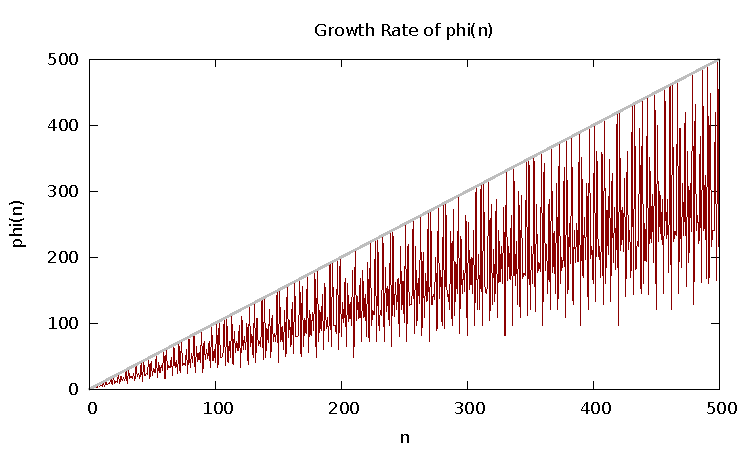
\includegraphics[scale=1]{eclipse/growth-rate.pdf}

\subsubsection{Geben Sie eine möglichst genaue obere Schranke für $\phi(n)$ an.}

\begin{align}
	 \phi(n) &\le n-1 \\
	 & \in \mathcal{O}(n)
\end{align}	
